\documentclass[11pt]{article}
\usepackage{mathtools}
\usepackage{amsmath}
\usepackage{amssymb}
\usepackage{amsfonts}
\usepackage{amsthm}
\usepackage{xcolor}
\usepackage{graphicx}
\usepackage[top=2.0cm,bottom=2.0cm,left=2.5cm,right=2.5cm]{geometry}
\usepackage{tikz}
\usepackage{float}
\usepackage{multicol}
\usepackage{pgfplots}
\usepackage{lastpage}
\usepackage{siunitx}
\usepackage{xspace}
\usepackage[labelfont=bf]{caption}
\usepackage[hidelinks, urlcolor=blue, linkcolor=blue, colorlinks=true]{hyperref}
\usepackage[capitalize,noabbrev]{cleveref}
\usepackage[absolute]{textpos}
\usepackage{systeme}

\newcommand{\R}{\mathbb{R}}
\newcommand{\C}{\mathbb{C}}
%% define course title
\newcommand{\course}{MAT185}
\newcommand{\assignmenttitle}{Assignment 1}

%% header and footer
\firstpageheader{}{}{\textbf{{\color{red} Due:} 10:00pm, Tuesday Jan. 21, 2025}}
\firstpageheadrule
\runningheader{}{Page~\thepage~of~\numpages}{\course~--~\assignmenttitle}
\footer{}{}{}

\setlength\parindent{0pt} % no indentation in document

%% formats exam class
\qformat{\textbf{Question \thequestiontitle:}\hfill} % title of question 
\boxedpoints
\pointpoints{mark}{marks}
\pointsinrightmargin
\hpword{Marks:}
\hsword{Your score:}
\unframedsolutions
\totalformat{\boxed{\textnormal{\totalpoints~\if\totalpoints1 mark\else marks\fi}}}
\definecolor{SolutionColor}{rgb}{0,0,1}
\renewcommand{\solutiontitle}{}
\AtBeginEnvironment{solution}{\color{blue}}

% %correct choices in solution
\CorrectChoiceEmphasis{\rm}
\checkedchar{\tikz\draw[blue,fill=blue] (0,0) circle (1ex);}

% % increase distance between checkbox items
\renewcommand{\checkboxeshook}{\setlength{\itemsep}{6pt}}

%% distance between questions and parts
\renewcommand{\questionshook}{\setlength{\parsep}{10pt}}
\renewcommand{\partshook}{\setlength{\parsep}{15pt}}

%% define arrows in text
\newcommand{\arrow}{$\rightarrow$\xspace}
\newcommand{\Arrow}{$\Rightarrow$\xspace}

% % math notation:
%\veccol{1}{2}{3}
\newcommand{\veccol}[3]{
    \begin{bmatrix}
        #1\\
        #2\\
        #3\\
    \end{bmatrix}}
  
%\vecrow{1}{2}{3}
\newcommand{\vecrow}[3]{\left[#1~#2~ #3\right]}

%\matrixTwo{1}{2}{3}{4}
\newcommand{\matrixTwo}[4]{\left[\begin{array}{cc}#1&#2\\#3&#4\end{array}\right]}

% \matrixThree{1}{2}{3}{4}{5}{6}{7}{8}{9}
\newcommand{\matrixThree}[9]{\left[\begin{array}{ccc}#1&#2&#3\\#4&#5&#6\\#7&#8&#9\end{array}\right]}

%\matrixCorner{1}{2}{3}{4}
\newcommand{\matrixCorner}[4]{\left[\begin{array}{ccc}#1& \cdots&#2\\ \vdots & \ddots & \vdots\\#3&
      \cdots&#4\end{array}\right]}

% \nR
\newcommand{\nR}{{}^{n}\mathbb{R}}
% \Rn
\newcommand{\Rn}{\mathbb{R}^{n}}
% \nRn
\newcommand{\nRn}{{}^{n}\mathbb{R}^{n}}
% \nRm
\newcommand{\nRm}{{}^{n}\mathbb{R}^{m}}
% \nRm
\newcommand{\mRn}{{}^{m}\mathbb{R}^{n}}
% \mRm
\newcommand{\mRm}{{}^{m}\mathbb{R}^{m}}        

% \u
\renewcommand{\u}{{\bf u}}      
% \v
\renewcommand{\v}{{\bf v}}      
% \w
\newcommand{\w}{{\bf w}}    
% \V
\newcommand{\V}{{\bf V}}                   
       
%% define abbreviations
\newcommand{\row}{\operatorname{row}\,}
\newcommand{\col}{\operatorname{col}\,}
\renewcommand{\dim}{\operatorname{dim}\,}
\renewcommand{\span}{\operatorname{span}\,}
\newcommand{\rank}{\operatorname{rank}\,}
\renewcommand{\ker}{\operatorname{ker}\,}
\newcommand{\nul}{\operatorname{null}\,}
\renewcommand{\det}{\operatorname{det}\,}
\newcommand{\adj}{\operatorname{adj}\,}

\usepackage{xcolor}
% Sean's original colours:
%\definecolor{dkrgreen}{rgb}{0.1, 0.4, 0.3} 
\definecolor{dkrgreen}{HTML}{009988} % this is the color-blind friendly teal from below
%\definecolor{dkred}{rgb}{0.8, 0.05, 0.05} 
\definecolor{dkred}{HTML}{EE3377}  % this is the colour-blind friendly magenta from below
%\definecolor{orange}{rgb}{0.8, 0.33, 0.0}
%\definecolor{goldenrod}{rgb}{0.85, 0.65, 0.13}
\definecolor{blue}{HTML}{1965B0} % this is the colour-blind friendly blue from below
%
% colour-blind-friendly colours from https://personal.sron.nl/~pault/
\definecolor{tolBlue}{HTML}{1965B0}
\definecolor{tolMedBlue}{HTML}{5289C7}
\definecolor{tolLightBlue}{HTML}{7BAFDE} 
\definecolor{tolRed}{HTML}{E8601C} 
\definecolor{tolYellow}{HTML}{F6C141}
\definecolor{tolTeal}{HTML}{009988}
%\definecolor{tolBlue}{HTML}{0077BB} 
\definecolor{tolCyan}{HTML}{33BBEE}
\definecolor{tolTeal}{HTML}{009988} 
\definecolor{tolOrange}{HTML}{EE7733} 
%\definecolor{tolRed}{HTML}{CC3311} 
\definecolor{tolMagenta}{HTML}{EE3377} 
\definecolor{tolGrey}{HTML}{BBBBBB}

%%% This command makes a framed box of a chosen height.
\newcommand{\makenonemptybox}[2]{%
\par\nobreak\vspace{\ht\strutbox}\noindent
\setlength{\fboxrule}{0pt} % set this to 0pt to make invisible
\fbox{%
\parbox[c][#1][t]{\dimexpr\linewidth-2\fboxsep}{
  \hrule width \hsize height 0pt
  \vspace{-0.6cm}
  \color{SolutionColor}#2\color{black}
 }%
}%
}


\begin{document}
\thispagestyle{empty}
{\LARGE \bf MSE 160 Lecture Notes}\\
{\large Hei Shing Cheung}\\
Molecules and Materials, Winter 2024 \hfill MSE 160\\
\\
The up-to-date version of this document can be found at \url{https://github.com/HaysonC/skulenotes}\\
\begin{center}
\textit{"In this class we are mostly understanding solids''} \\ - Prof. \textsc{Scott Ramsay}
\end{center}
\vspace{10pt}
\section{Mechanical Behavior}
\paragraph{Classes of Materials} In this class, we look at three classes of materials (non-exhaustive):
\begin{itemize}
    \item \textbf{Metal} held together with metallic bonds, typically \textbf{ductile} and \textbf{conductive}.
    \item \textbf{Ceramics}  (often metal oxides [excp: diamond]) held together via covalent \& ionic bonds, typically \textbf{brittle} and \textbf{insulating}.
    \item \textbf{Polymers} Molecules (often hydrocarbons) typically \textbf{ductile} and \textbf{insulating}
\end{itemize}
\paragraph{Engineering Stress} For normal stress, we know that:
\begin{equation}
    \sigma = \frac{F}{A_0}
\end{equation}
\paragraph{Engineering Strein} Also:
\begin{equation}
    \epsilon = \frac{\Delta l}{l_0}
\end{equation}
\paragraph{Young's Moduclus} For elastic deformation, $E$, is given, by Hooke's Law, as follows:
\begin{equation}
    \sigma = E \epsilon
\end{equation}
\paragraph{Tensile Test} We apply force as to the ends of a dogbone-sample, with $l_0$ being the gauge length and $A_0$ being the area of the cross-section at the middle. 
\paragraph{Tensile Strein} Maximum tensile strain on the engineeging stress-strain curve.
\subsection{Understanding Elastic Properties in terms of Atomic Configuration}
\paragraph{Atomic Configuration} We can understand the elastic properties of a material by looking at the atomic configuration. Skemetically, we can represent the atomic configuration as a spring system:
\begin{enumerate}
    \item \textbf{Intial - Before Loading} Atoms are in equilibrium, with the interatomic forces being balanced.
    \item \textbf{Loading} We apply a force to the material, causing the atoms to move from their equilibrium positions. The bond stretches and the atoms move further apart.
    \item \textbf{Unloading} We remove the force, causing the atoms to return to their equilibrium positions. 
\end{enumerate}
\paragraph{Atom Positions} Elastic modulus is dependent on the atomic interatomic bonding force. Thus, The elastic modulus is prootionaly to the slope of the interatomic force-seperation curve.
\paragraph{Force-Seperation Curve} The force-seperation curve is a plot of the force between two atoms as a function of the distance between them. The slope of the curve is proportional to the elastic modulus near the equilibrium position.

\begin{figure}[h]
    \centering
    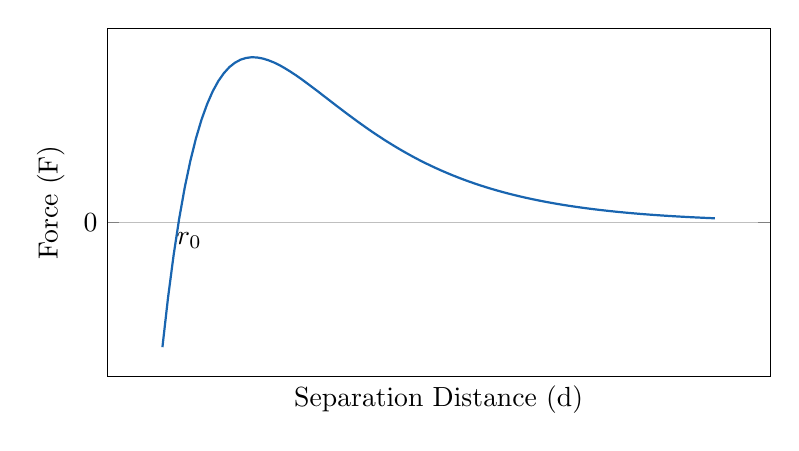
\begin{tikzpicture}
        \begin{axis}[
            xlabel={Separation Distance (d)},
            ylabel={Force (F)},
            grid=major,
            width=10cm,
            height=6cm,
            domain=-0.3:10,
            samples=100,
            xtick = \empty,
            ytick = {0}
        ]
        \addplot[blue, thick] {exp(-x/2) - exp(-x)};
        \node at (axis cs:0.2,0) [anchor=north] {$r_0$};
        
    \end{axis}
    \end{tikzpicture}
    \caption{Force-Separation Curve (Lennard-Jones Force)}
    \label{fig:force-separation}
\end{figure}
\begin{equation}
    E \propto \frac{dF}{dr} \Bigg|_{r_0}
\end{equation}
\begin{definition}[Equilibrium interatomic seperation distance]
The equilibrium interatomic seperation distance, $r_0$, is the distance between two atoms at which the interatomic force is zero. This is due to the interatomic forces being the sum of attractive and repulsive forces.
\end{definition}
\paragraph{Elastic Modulus} Thus, strongly bonded materials have a higher elastic modulus and the slope of the force-seperation curve is steeper at $r_0$.
\subsection{Understanding Other Properties in terms of Atomic Configuration}
\paragraph{Potential Energy-Separation Curve} The potential energy-seperation curve is a plot of the potential energy between two atoms as a function of the distance between them. The potential energy is the area under the force-seperation curve.
\paragraph{Depth of the Minimum Energy Well} The depth of the minimum energy well, $E_0$, is the energy required to break the bond between two atoms. This is the energy required to move the atoms from the equilibrium position to infinity. It is proportional to the melting temperature of the material.
\begin{figure}[h]
    \centering
    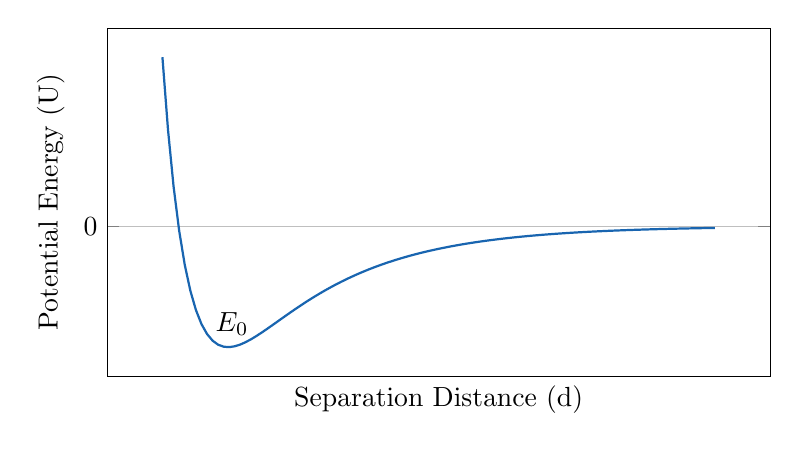
\begin{tikzpicture}
        \begin{axis}[
            xlabel={Separation Distance (d)},
            ylabel={Potential Energy (U)},
            grid=major,
            width=10cm,
            height=6cm,
            domain=-0.3:10,
            samples=100,
            xtick = \empty,
            ytick = {0}
        ]
        \addplot[blue, thick] {-exp(-x/2) + exp(-x)^2};
        \node at (axis cs:1,-0.3) [anchor=north] {$E_0$};
        
    \end{axis}
    \end{tikzpicture}
    \caption{Potential Energy-Separation Curve}
    \label{fig:potential-energy}
\end{figure}
\paragraph{Coefficient of Thermal Expansion} The coefficient of thermal expansion, $\alpha$, is the fractional change in length per degree change in temperature. 
\paragraph{Depth of Potential Energy Curve} The deeper the potential energy curve, the higher the melting temperature and more symetric the curve near $E_0$. This would give the follwoing three properties:
\begin{enumerate}
    \item \textbf{Higher Melting Temperature} The higher the melting temperature, the deeper the potential energy curve.
    \item \textbf{Higher Elastic Modulus} The steeper the slope of the force-seperation curve at $r_0$, the higher the elastic modulus.
    \item \textbf{Lower Coefficient of Thermal Expansion} The more symetric the potential energy curve near $E_0$, the lower the coefficient of thermal expansion.
\end{enumerate}
\subsection{Shear and Tensile Stress}
\subsubsection{Shear}
\paragraph{Shear Stress} Shear stress is the force per unit area acting parallel to the surface. It is given by:
\begin{equation}
    \tau = \frac{F}{A_0}
\end{equation}
\paragraph{Shear Strain} Shear strain is the change in angle between two lines originally perpendicular to each other. It is given by:
\begin{equation}
    \gamma = \frac{\Delta l}{l_0} \approx \tan \theta \approx \theta = \frac{\pi}{2} - \phi
\end{equation}
\paragraph{Shear Modulus} The shear modulus, $G$, is the ratio of shear stress to shear strain. It is given by:
\begin{equation}
    \tau = G \gamma
\end{equation}
\paragraph{Relationship between Shear and Tensile Modulus} The shear modulus is related to the tensile modulus by the following equation:
\begin{equation}
    G = \frac{E}{2(1+\nu)}
\end{equation}
where $\nu$ is the Poisson's ratio.
\paragraph{Poisson's Ratio} Poisson's ratio, $\nu$, is the ratio of lateral strain to axial strain. It is given by:
\begin{equation}
    \nu = -\frac{\epsilon_{\text{lat}}}{\epsilon_{\text{axial}}}
\end{equation}
\subsection{Testing}
\begin{definition}[Gauge Length]
The gauge length, $l_0$, is the length of the sample over which the strain is measured.
\end{definition}
\begin{definition}[Reduced Section]
The reduced section is the part of the sample where the cross-sectional area is reduced to a smaller value.
\end{definition}
\paragraph{} Gauge length is always no longer than the reduced section. The reduced section is where the sample will likely break.
\paragraph{Testing Ceremics} In relation to tensile testing, ceramics have the following properties:
\begin{itemize}
    \item \textbf{Brittle} Ceramics are brittle and will break suddenly.
    \item \textbf{High Strength} Ceramics have high strength and thus difficult to machine the sample.
    \item \textbf{Sample Alignment} The sample must be aligned properly to test for pure tension. Unlike metals and polymers, which are self-aligning.
    \item \textbf{Fracture} Ceramics will fracture while still off-axis. Hence, there would be a large shear component. 
\end{itemize}
\paragraph{} Thus, we often approxiate tensile behaviour with a point loading on a horizontal beam, with two point support (3 point bending test). Peak stress is given by:
\begin{equation}
    \sigma_{\text{peak}} = \frac{3FL}{2bd^2}
\end{equation}
, where:
\begin{itemize}
    \item $L$ (span) is the distance between the two supports.
    \item $b$ is the width of the sample
    \item $d$ is the thickness/depth of the sample
\end{itemize}
\section{Seleection of Materials}
\subsection{Material Performance}
\begin{example}[Aircraft Wing Spar]
    The aircraft wing spar is beam (loaded in bending) that supports the wing. The spar is made of a material with the objective of minimize mass under the following constraints:
    \begin{itemize}
        \item \textbf{Deflection} There is a maximum allowable deflection of the wing.
        \item There is more..., but for this example, we will only consider the deflection.
    \end{itemize}
    The material selection solve for a \textbf{light stiff beam}.

    \paragraph{Mass} The mass of the beam is given by:
    $$ m = \rho V = \rho A L $$
    \paragraph{Deflection} The deflection of the beam is given by:
    \begin{equation}
        \delta = \frac{FL^3}{48EI} 
    \end{equation}
    \begin{align*} 
        \intertext{For a beam with a rectangular cross-section, we have:}
        \delta &= \frac{FL^3}{48E} \cdot \frac{12}{bh^3} = \frac{FL^3}{4Ebh^3}  
        \intertext{We can set $b$ proportional to $h$:}
        \delta &= \frac{FL^3}{cE} \cdot \frac{1}{A^2},\quad \text{for some constant $c$} 
        \intertext{We can then isolate for $A$, the free variable, and minimize the mass via the objective equation $m = \rho A L$:}
        A &= \sqrt{\frac{FL^3}{cE\delta}} \\
        m &= \rho L \sqrt{\frac{FL^3}{cE\delta}} = \rho L \sqrt{\frac{FL^3}{cE\delta}}
        \intertext{Arrange into the form (functional)(geometric)(material):}
        m &= \left(\frac{F}{c\delta}\right)^\frac{1}{2} \cdot \left(L^\frac{5}{2}\right)\cdot\left(\frac{\rho}{E^\frac{1}{2}}\right)
    \end{align*}
\end{example}
\paragraph{Material Peformance Index} The material performance index is given by:
    \begin{equation}
        \text{Material Performance Index (MSI)} = \frac{E^\frac{1}{2}}{\rho}
\end{equation}
\paragraph{MPI Graph} We plot $\log E$ against $\log \rho$ to get the MPI graph. 
\paragraph{Tempered Glass} Temperglass are made to resist tension. It is done by applying a compressive stress to the surface of the glass. This is done by cooling the surface of the glass faster than the core or chemically treating the surface.
\subsection{Density}
\paragraph{Density} The density of a material is given by:
\begin{equation}
    \rho = \frac{m}{V}
\end{equation}
\paragraph{Archimedes' Principle} The buoyant force on an object is equal to the weight of the fluid displaced by the object. Derive from that, we have:
\begin{equation}
    \rho = \frac{m}{V} = \frac{m_{\text{object}}}{m_{\text{object}} - m_{\text{object in fluid}}}
\end{equation}
\section{Atomic Structures}
\subsection{General Definitions}
\paragraph{Ordered structures} We have the following three orders:
\begin{enumerate}
    \item \textbf{Long Range Order (LRO)} Atoms are arranged in a well-defined pattern over long distances in repeating units. \\
    (Example) Diamonds, some polymers, most metals, many ceramics, graphite, quartz, etc.
    \item \textbf{Short Range Order (SRO)} Periodic arrangement of atoms over a few atomic or molecular spacings. \\
    (Example) Most polymers, glasses, amorphous materials, etc.
    \item \textbf{No Order (NO)} Atoms are randomly arranged. \\
    (Example) Ideal gases, etc.
\end{enumerate}
\paragraph{Describing Crystal Structures} We can describe crystal structures by the following:
\begin{itemize}
    \item \textbf{Unit Cell} The smallest repeating unit of a crystal structure that could be used to represent the entire crystal.
    \item \textbf{Lattice} The repeating arrangement of points that repersent the positions of atoms in the unit cell.\\
    (Example) Simple Cubic, Body-Centered Cubic, Face-Centered Cubic, etc.
    \item \textbf{Lattice Plus Basis} \textit{Not required for this course}
\end{itemize}
\paragraph{Theortical Density of Metals} The theoretical density of metals is given by:
\begin{equation} \label{eq:theoretical-density}
    \rho = \frac{nM}{V_c N_A}
\end{equation}
, where:
\begin{itemize}
    \item $n$ is the number of atoms in the unit cell.
    \item $M$ is the atomic mass of the element (amu = g/mol).
    \item $V_c$ is the volume of the unit cell.
    \item $N_A$ is Avogadro's number ($6.022 \times 10^{23} \text{mol}^{-1}$)
\end{itemize}
\subsection{Describing Basic Unit Cells}
\begin{definition}[Coordination Number (CN)]
    The coordination number is the number of nearest neighbors an atom has in a crystal structure.
\end{definition}
\begin{definition}[Atomic Packing Factor (APF)]
    The atomic packing factor is the fraction of the volume of the unit cell that is occupied by hard spheres. It is given by:
    \begin{equation}
        \text{APF} = \frac{\text{Volume of atoms in unit cell}}{\text{Volume of unit cell}}
    \end{equation}
\end{definition}
\paragraph{Simple Cubic (SC)} The simple cubic structure has the following properties:
\begin{itemize}
    \item \textbf{Centers of atoms} Located at the eight corners of a cube
    \item \textbf{Rare Packing Density}  Due to low packing density (only known example: Polonium, Po)
    \item \textbf{Close-packed directions} As cube edges.
    \item \textbf{Coordination Number} Number of nearest neighbor: 6
\end{itemize}
\paragraph{Face-Centered Cubic (FCC)} The face-centered cubic structure has an atom on the centre of each face of the cube. It has the following properties:
\begin{itemize}
    \item \textbf{Ductile} and \textbf{Malleable} due to the close-packed planes. Common examples include: \\ $\ch{Al}\, ,\ch{Cu}\, ,\ch{Au}\, ,\ch{Ag}$.
    \item \textbf{Coordination Number} Number of nearest neighbor: 12
    \item \textbf{Close-packed directions} As cube diagonals.
    \item \textbf{Theortical Density} The theoretical density of FCC is derived from Equation (\ref{eq:theoretical-density}):
    \begin{align}
        \rho &= \frac{nM}{V_c N_A} \nonumber \\
        \intertext{With $n = 4$ (8 corners $\times \frac{1}{8}$ atom each + 6 faces $\times \frac{1}{2}$ atom each) and $V_c = a^3$ (where $a$ is the \textbf{lattice parameter}):}
        \rho_\text{FCC} &= \frac{4M}{a^3 N_A} \nonumber \\
        \intertext{We can then obtain $a$ via the relationship between the atomic radius, $r$, and the lattice parameter via the geometry on the close-packed direction (face diagonal):}
        a &= 2\sqrt{2}r \nonumber \\
        \intertext{Substitute $a$ back into the equation:}
        \rho_\text{FCC} &= \frac{4M}{(2\sqrt{2}r)^3 N_A} = \frac{4M}{16\sqrt{2}r^3 N_A} \nonumber \\
        &= \frac{M}{4\sqrt{2}r^3 N_A} 
    \end{align}
    \item \textbf{Atomic Packing Factor} The atomic packing factor of FCC is given by:
    \begin{equation}
        \text{APF}_\text{FCC} = \frac{\text{Volume of atoms in unit cell}}{\text{Volume of unit cell} } = \frac{4 \times \frac{4}{3}\pi r^3}{a^3} = \frac{4 \times \frac{4}{3}\pi r^3}{(2\sqrt{2}r)^3} = \frac{\pi}{6\sqrt{2}} = \textbf{0.74}
    \end{equation}
    This is the highest possible packing factor for spheres. Thus, no other structure can have a higher packing factor.
    \item \textbf{Stacking} The FCC structure can be thought of as stacking close-packed planes. The stacking sequence is ABCABC... (where A, B, and C describe the orientation hexagonal close-packed planes).
\end{itemize}
\paragraph{Hexagonal Close-Packed (HCP)} The hexagonal close-packed structure is \textbf{crytal structure} by stacking close-packed hexagonal planes. It has the following properties:
\begin{itemize}
    \item \textbf{Coordination Number} Number of nearest neighbor: 12
    \item \textbf{Close-packed directions} As cube diagonals.
    \item \textbf{Theortical Density} The theoretical density of HCP is derived from Equation (\ref{eq:theoretical-density}):
    \begin{align}
        \rho &= \frac{nM}{V_c N_A} \nonumber \\
        \intertext{With $n = 6$ (12 corners $\times \frac{1}{6}$ atom each) and $V_c = a^3$:}
        \rho_\text{HCP} &= \frac{6M}{a^3 N_A} 
    \end{align}
    \item \textbf{Atomic Packing Factor} The atomic packing factor of HCP is given by:
    \begin{equation}
        \text{APF}_\text{HCP} = \frac{\text{Volume of atoms in unit cell}}{\text{Volume of unit cell} } = \frac{6 \times \frac{4}{3}\pi r^3}{a^3} = \frac{6 \times \frac{4}{3}\pi r^3}{a^3} = \textbf{0.74}
    \end{equation}
    \item \textbf{Stacking} The HCP structure can be thought of as stacking close-packed planes. The stacking sequence is ABAB...
\end{itemize}
\begin{example}[Density of Aluminum]
    Given that the atomic radius of aluminum is $r = 143$ pm and the atomic mass is $M = 26.98$ g/mol, we can calculate the density of aluminum with FCC structure. We have:
    \begin{align*}
        \rho_\text{Al} &= \frac{M}{4\sqrt{2}r^3 N_A} = \frac{26.98}{4\sqrt{2} \times (143 \times 10^{-12})^3 \times 6.022 \times 10^{23}} \\
        &= \frac{26.98}{4\sqrt{2} \times (143 \times 10^{-12})^3 \times 6.022 \times 10^{23}} = 2.7 \text{ g/cm}^3
    \end{align*}
\end{example}
\paragraph{Body-Centered Cubic (BCC)} The body-centered cubic structure has an atom at the centre of the cube. It has the following properties:
\begin{enumerate}
    \item \textbf{Coordination Number} Number of nearest neighbor: 8
    \item \textbf{Atomic Packing Factor} The atomic packing factor of BCC is given by:
    \begin{equation}
        \text{APF}_\text{BCC} = \frac{\text{Volume of atoms in unit cell}}{\text{Volume of unit cell} } = \frac{2 \times \frac{4}{3}\pi r^3}{a^3} = \frac{2 \times \frac{4}{3}\pi r^3}{(4r/\sqrt{3})^3} = \textbf{0.68}
    \end{equation}
    \item \textbf{Close Packed Directions} As cube diagonals.
    \item \textbf{Theortical Density} The theoretical density of BCC is derived from Equation (\ref{eq:theoretical-density}):
    \begin{align}
        \rho &= \frac{nM}{V_c N_A} \nonumber \\
        \intertext{With $n = 2$ (8 corners $\times \frac{1}{8}$ atom each + 1 center atom) and $V_c = a^3$:}
        \rho_\text{BCC} &= \frac{2M}{a^3 N_A} 
    \end{align}
    \item \textbf{Stacking} The BCC structure can be thought of as stacking close-packed planes. The stacking sequence is ABAB...
\end{enumerate}
\section{Geometric Properties of Crystals}
\subsection{Crystallographic Directions and Planes}
\paragraph{Point Coordinates} A lattice positon in a unit cell is determined as fractional multiples of the unit cell edge lengths $a$, $b$, and $c$. (Defining the origin at one corner of the unit cell and $a=b=c=\textbf{1}$)
\paragraph{Crystallographic Directions} A crystallographic direction is a line between two points in a crystal. It is denoted by square brackets, $[uvw]$. The direction is determined from the ``tail'' to the ``head'' of the vector. Also:
\begin{enumerate}
    \item It \textbf{shall not} include commas; and
    \item It \textbf{shall be reduced}to the smallest integers; and
    \item Negative signs are represented by a bar over the number.
\end{enumerate}
\begin{example}
    The crystallographic direction from $(0,0,0)$ to $(-1,0,1/2)$ is $[\bar{2}01]$.
\end{example}
\paragraph{Family of Directions} A family of directions is a set of directions that are parallel to each other. It is denoted by $<uvw>$.
\begin{example}
    The family of directions $<100>$ is the set of directions $[100]$, $[010]$, $[001]$, $[\bar{1}00]$, $[0\bar{1}0]$, and $[00\bar{1}]$.
\end{example}
\paragraph{Angle between Directions} The angle between two directions in a \textbf{cubic} crystal is given by:
\begin{equation}
    \cos \theta = \frac{h_1h_2 + k_1k_2 + l_1l_2}{\sqrt{h_1^2 + k_1^2 + l_1^2}\sqrt{h_2^2 + k_2^2 + l_2^2}}
\end{equation}
, which is simply the normalized dot product of the two vectors.
\paragraph{Crystallographic Planes} A crystallographic plane is a set of parallel planes in a crystal. It is denoted by $(hkl)$. The plane is determined by the intercepts on the $x$, $y$, and $z$ axes. 
\paragraph{} Generally, we find the intercepts by finding the points where the plane intersects the axes. We then take the reciprocals of the intercepts and multiply by the smallest integer to get the Miller Indices.
\paragraph{Family of Planes} A family of planes is a set of planes that are parallel to each other. It is denoted by $\{hkl\}$.
\paragraph{Distance between Planes} The distance between two planes with miller indices $(h_1k_1l_1)$ and $(h_2k_2l_2)$ is given by:
\begin{equation}
    d = \frac{a}{\sqrt{h^2 + k^2 + l^2}}
\end{equation}
, where $a$ is the lattice parameter.
\subsection{X-Ray Diffraction} The diffraction pattern is used to determine the crystal structure. By measuring the n$^\text{th}$ order peak angle $\theta_c$ and the wavelength of the X-ray, we can determine the distance between planes:
\begin{align}
    2d\sin \theta &= n\lambda \nonumber \\
    d &= \frac{n\lambda}{2\sin \theta_c}
    \intertext{Thus, we could determine the lattice parameter $a$ by the following equation:}
    a &= \frac{n\lambda}{2\sin \theta_c} \sqrt{h^2 + k^2 + l^2}
\end{align}

\includepdf[pages=-, angle=90]{EquationSheet.pdf}
\end{document}
